\documentclass[11pt]{article}
\usepackage[margin=0.8in]{geometry}
\usepackage[]{amsfonts, amssymb, amsmath, float, hyperref,fancyheadings, graphicx, derivative}
\pagestyle{fancy}
\lhead{Machine Learning}
\chead{Larry128}
\rhead{COMP4211}
\renewcommand{\footrulewidth}{0.4pt}
\setcounter{tocdepth}{3} % set TOC
\newcommand{\indep}{\perp \!\!\! \perp}

% codeblocks
\usepackage{listings}
\usepackage{xcolor}
\definecolor{codegreen}{rgb}{0,0.6,0}
\definecolor{codegray}{rgb}{0.5,0.5,0.5}
\definecolor{codepurple}{rgb}{0.58,0,0.82}
\definecolor{backcolour}{rgb}{0.95,0.95,0.92}
\lstdefinestyle{mystyle}{
    backgroundcolor=\color{backcolour},   
    commentstyle=\color{codegreen},
    keywordstyle=\color{magenta},
    numberstyle=\tiny\color{codegray},
    stringstyle=\color{codepurple},
    basicstyle=\ttfamily\footnotesize,
    breakatwhitespace=false,         
    breaklines=true,                 
    captionpos=b,                    
    keepspaces=true,                 
    numbers=left,                    
    numbersep=5pt,                  
    showspaces=false,                
    showstringspaces=false,
    showtabs=false,                  
    tabsize=3
}
\lstset{style=mystyle}
\lstdefinestyle{customc}{
  language=C++,
  % Add other settings here
}

%common math symbols
\newcommand{\R}{\mathbb{R}}
\newcommand{\N}{\mathbb{N}}
\newcommand{\Q}{\mathbb{Q}}
\newcommand{\ddx}{\dfrac{d}{dx}}
\newcommand{\regressf}{$f(\mathbf{x}; \mathbf{w})$ }
\newcommand{\lossf}{$L(\mathbf{w}; S)$ }

% asymptotic notations
\newcommand\BigO[1]{$O($#1$)$}
\newcommand\BigOmega[1]{$\Omega($#1$)$}
\newcommand\BigTheta[1]{$\Theta($#1$)$}
\newcommand\pddx[2]{\frac{\partial{#1}}{\partial{#2}}}

% pgfplots
\usepackage{pgfplots}
\pgfplotsset{compat=1.18, width=8cm}
\usepackage{geometry}
\geometry{
a4paper,
total={170mm,257mm},
left=20mm,
top=20mm,
}
\usepackage{algorithm}
\usepackage{algpseudocode}

\begin{document}
\begin{titlepage}
    \begin{center}
        \vspace*{1cm}
            
        \Huge
        \textbf{COMP4211}
            
        \vspace{0.5cm}
        \LARGE
        Machine Learning
            
        \vspace{1.5cm}
            
        Larry128
            
        \vfill
            
        A summary notes for revision
            
        \vspace{0.8cm}
                
        \Large
        Fall 2024-2025
            
    \end{center}
\end{titlepage}

\tableofcontents
\newpage

\section{Linear Regression}
\subsection{Basic Ideas of Regression}
\begin{enumerate}
\item Given a training set $S = \{(x^{(l)}, y^{(l)})\}_{l=1}^{N}$ of $N$ labelled examples of input-output pairs.
\item A \textbf{Regression Function} \regressf uses $S$ such that the predicted output $f(\mathbf{x^{(l)}}; \mathbf{w})$ for each input $\mathbf{x}^{l}$ such that $f(\mathbf{x}^{(l)}; \mathbf{w}) \approx \mathbf{y}^l$.
\item (multi-output regression) When the output $\mathbf{y}$ is a vector, it's a multi-output regression.
\item We denote the output by $y$ if the output is univariate.
\item The input $\mathbf{x} = (x_1 , \cdots, x_d) ^T$ is $d$-dimensional.
\end{enumerate}

\subsection{Linear Regression Function}
\begin{enumerate}
\item If the regression function is linear, then 
\begin{align*}
f(\mathbf{x}; \mathbf{w}) &= w_{0} + w_1 x_1 + \cdots + w_d x_d\\
&= \begin{bmatrix}
w_0& w_1& \cdots& w_d
\end{bmatrix} \begin{bmatrix}
1\\
x_1\\
\vdots\\
x_d
\end{bmatrix} &= \begin{bmatrix}
1 & x_1& \cdots& x_d
\end{bmatrix} \begin{bmatrix}
w_0\\
w_1\\
\vdots\\
w_d
\end{bmatrix}\\
&= \mathbf{w}^{T} \mathbf{\tilde{x}} &= \mathbf{\tilde{x}}^{T} \mathbf{w}
\end{align*}
\item $w_0$ is the \textit{bias} term which serves as an offset.
\item The learning problem is to find the best $\mathbf{w}$ according to performance measure on $S$.
\end{enumerate}

\subsection{Loss Function}
\begin{enumerate}
\item A common way to learn the parameter $\mathbf{w}$ of \regressf is to define a loss function \lossf
\item The most common loss function is the \textbf{squared loss}
\begin{align*}
L(\mathbf{w}; S) &= \sum_{l=1}^{N} (f(\mathbf{x}^{(l)} ;\mathbf{w})- \mathbf{y}^{(l)})^2\\
&= \sum_{l=1}^{N} (w_0 + w_1 x_1 ^{(l)}+ \cdots + w_d x_d ^{(l)} - y^{(l)})^2
\end{align*}
\item We may also define the loss function by \textbf{mean} rather than the sum $$L(\mathbf{w}; S) = \dfrac{1}{N} \sum_{l=1}^{N} (f(\mathbf{x}^{(l)} ;\mathbf{w})- \mathbf{y}^{(l)})^2$$
\item A special case ($d=1$)\\
Squared loss: $$L(\mathbf{w}; S) = \sum_{l=1}^{N}(w_0 +w_1 x_1 ^{(l)} - y^{(l)})^2$$
We can find the unique optimal solution $\tilde{\mathbf{w}} = \begin{bmatrix}
w_0\\w_1
\end{bmatrix}$ that minimizes \lossf using the method of least squares.\\
First, we take the derivatives of \lossf with respect to $w_0$ and $w_1$ and set them to $0$.
\begin{align*}
\pddx{L}{w_0} &= 2\sum_{l=1}^{N} (w_0 +w_1 x_1 ^{(l)} - y^{(l)}) =0  \iff \sum_{l=1}^{N}(w_0 +w_1 x_1 ^{(l)}) = \sum_{l=1}^{N} y^{(l)} \iff N w_0 + \sum_{l=1}^{N} w_1 x_1 ^{(l)} = \sum_{l=1}^{N} y^{(l)}\\
\pddx{L}{w_1} &= 2\sum_{l=1}^{N} (w_0 +w_1 x_1 ^{(l)} - y^{(l)})x_1 ^{(l)}=0 \iff w_0 \sum_{l=1}^{N} x_1 ^{(l)} + w_1 \sum_{l=1}^{N} (x_{1}^{(l)})^2 = \sum_{l=1}^{N}x_1 ^{(l)} y^{(l)}
\end{align*}
Then, we have a system of linear equations of two unknown $w_0$, $w_1$. We can write it in matrix form.
\begin{align*}
\mathbf{A} \mathbf{w} = \begin{bmatrix}
N &\sum_{l} x_{1} ^{l}\\
\sum_{l} x_{1} ^{l} &\sum_{l} (x_{1} ^{l})^2
\end{bmatrix} \begin{bmatrix}
w_0\\w_1
\end{bmatrix} = \begin{bmatrix}
\sum_{l} y^{(l)}\\ \sum_{l} x_1 ^{(l)} y^{(l)}
\end{bmatrix} = \mathbf{b}
\end{align*}
Assuming $\mathbf{A}$ is invertible, the least squares estimate is $$\tilde{\mathbf{w}} = \mathbf{A}^{-1} \mathbf{b}$$

\item General case ($d \geq 1$)
\begin{enumerate}
\item (First approach) We express the input and output of $N$ examples as follows
\begin{align*}
\mathbf{X} = \begin{bmatrix}
1& x_1 ^{l}&\cdots & x_{d}^{1}\\
1& x_1 ^{2}&\cdots & x_{d}^{2}\\
\vdots\\
1& x_1 ^{N}&\cdots & x_{d}^{N}
\end{bmatrix}, &&\mathbf{y} = \begin{bmatrix}
y^{(1)}\\
y^{(2)}\\
\vdots\\
y^{(N)}
\end{bmatrix}
\end{align*}
Then we can express the matrix form as follows (proof skipped)
$$\mathbf{A w = X^T X w = X^T y = b}$$
Therefore, the least squares estimate is $$\tilde{\mathbf{w}} = \mathbf{(X^T X)^{-1} X^T y}$$, assuming $\mathbf{X^T X}$ is invertible
\item (Second approach) First write $\mathbf{X w - y}$ as
\begin{align*}
\mathbf{Xw - y} &= \begin{bmatrix}
1& x_1 ^{l}&\cdots & x_{d}^{1}\\
1& x_1 ^{2}&\cdots & x_{d}^{2}\\
\vdots\\
1& x_1 ^{N}&\cdots & x_{d}^{N}
\end{bmatrix} \begin{bmatrix}
w_0\\
w_1\\
\vdots\\
y_d
\end{bmatrix} - \begin{bmatrix}
y^{(1)}\\
y^{(2)}\\
\vdots\\
y^{(N)}
\end{bmatrix}\\
&= \begin{bmatrix}
w_0 + w_1 x_1 ^{(1)} + \cdots + w_d x_d ^{1} - y^{(1)}\\
w_0 + w_1 x_1 ^{(2)} + \cdots + w_d x_d ^{2} - y^{(2)}\\
\vdots\\
w_0 + w_1 x_1 ^{(N)} + \cdots + w_d x_d ^{N} - y^{(N)}\\
\end{bmatrix}
\end{align*}
Then the squared loss is just the square of \textbf{L-2 norm} of $\mathbf{Xw -y}$ $$L(\mathbf{w}; S) = ||\mathbf{Xw - y}||^2$$
We can further write the squared loss as
\begin{align*}
L(\mathbf{w}; S) &= ||\mathbf{Xw - y}||^2\\
&= (\mathbf{Xw - y})^T (\mathbf{Xw - y})\\
&= (\mathbf{w^T X^T - y^T})(\mathbf{Xw - y})\\
&= \mathbf{w^T X^T X w - 2 y^T X w + y^T y}
\end{align*}
After that, we can take the derivative with respect to $\mathbf{w}$ \begin{align*}
&\pddx{L}{\mathbf{w}} = 2 \mathbf{X^T X w} - 2 \mathbf{X^T y} =0\\
\iff& \mathbf{X^T X w} = \mathbf{X^T y}\\
\iff& \tilde{\mathbf{w}}= \mathbf{(X^T X)^{-1} X^T y}
\end{align*}
\item Complexity considerations\\
To compute $\tilde{\mathbf{w}}$, we need to invert $\mathbf{X^T X} \in \mathbb{R}^{(d+1) \times (d+1)}$. $Le Gall$ is the fastest algorithm to compute that with $O(n^{2.3728639})$, instead of $O(n^3)$ for Cholesky, LU, Gaussian elimination.
\end{enumerate}
\subsection{Non-linear Extensions}
\begin{enumerate}
\item For solving more complicated problems, non-linear regression function are needed.
\item Different approaches for non-linear extension are:
\begin{enumerate}
\item Explicitly adding more input dimensions (which depend non-linearly on the original input dimensions) and applying linear regress to the expanded input. Here is an example
$$f(\mathbf{x}; \mathbf{w}) = w_0 \cdot 1 + w_1 x_1 + w_2 x_2 +\cdots + w_d x_d + w_{d+1} x_1^{2} x_8^{3} + w_{d+2} x_{10} x_{19} $$ In this case, $$\mathbf{\tilde{x}} = \begin{bmatrix}
1\\x_1 \\ \vdots \\ x_d \\ x_1^{2} x_8^{3} \\ x_{10} x_{19}
\end{bmatrix}, \mathbf{w} = \begin{bmatrix}
w_0\\ w_1 \\ \vdots \\ w_{d} \\ w_{d+1} \\ w_{d+2}
\end{bmatrix}$$
\item Applying an explicit defined non-linear regression function to the original input. For example $$f(\mathbf{x}; \mathbf{w}) = w_0 + w_1 x_1 x_2 ^2 + w_2 x_3 x_5 ^8 + \cdots$$
\item Applying an implicitly defined non-linear transformation to the original input and then a linear model to the transformed input $$ U \mapsto V, \mathbf{x} \in U, \mathbf{z} \in V, f(\mathbf{z}; \mathbf{w})$$
\end{enumerate}
\item We will consider the first approach here and leave the other two for some later topics
\item Advantage of the first approach is that linear regression can still be used and the weights in a linear regression model have \textbf{text interpretability} (the larger the magnitude of a weight, the more significant is the corresponding input feature).
\item (Polynomial Regression). One common approach is to introduce \textit{higher-order terms} as additional input dimensions, e.g., $x_i ^2, x_i x_j, x_i x_j ^2 x_k$
\begin{align*}
f(\mathbf{x}; \mathbf{w}) &= w_0 +w_1 x+ \cdots+ w_m x^m\\
&= \begin{bmatrix}
w_0 & w_1 & \cdots & w_m
\end{bmatrix}\begin{bmatrix}
1\\ x\\ \vdots \\ x^m
\end{bmatrix}\\
&= \mathbf{w}^T \mathbf{\tilde{x}}
\end{align*}
Remark: Although $f$ is non-linear in $\mathbf{\tilde{x}}$, it is linear in the optimization variable $\mathbf{w}$.\\
Very often, \textbf{feature engineering} that uses domain knowledge to define application-specific features is applied, two of the original features are body weight and body height, we may define the body mass index (BMI)
\end{enumerate}
\end{enumerate}
\subsection{Model Over-fitting}
\begin{enumerate}
\item If the training set $S = \{(\mathbf{x}^{l}, \mathbf{y}^{l})\}_{l=1}^N$ is small compared to the number of parameters in the linear regression function $f(\mathbf{x}; \mathbf{w})$, overfitting may occur.
\item When overfitting occurs, it is common to find large magnitudes in at least some of the parameters. This is because a large search space is needed for the (overly complex) model to fit the data exactly.
\item One common solution to the overfitting problem is to prevent the parameters from growing excessively large in magnitude.
\begin{align*}
\text{Overfitting} &\implies \text{Large magnitudes in some weights}\\
\equiv \text{Not large magnitudes in some weights} &\implies \text{Not overfitting}
\end{align*}
To attain so, we will do \textbf{Regularization}.
\end{enumerate}
\subsection{Regularization}
\begin{enumerate}
\item Regularization is an approach which modifies the original loss function by adding one or more penalty terms, called regularizers, that penalize large parameter magnitudes. 
\item For example, Regularized loss function based on $L_2$ regularization (a.k.a. Tikhonov regularization)
\begin{align*}
L_{\lambda} (\mathbf{w}; S) &= L(\mathbf{w}; S) + \lambda ||\mathbf{w}||^2\\
&= ||\mathbf{Xw-y}||^2 + \lambda ||\mathbf{w}||^2\\
&= (\mathbf{Xw-y})^T (\mathbf{Xw-y}) + \lambda \mathbf{w}^T \mathbf{w}\\
&= \mathbf{w}^T \mathbf{X}^T \mathbf{X} \mathbf{w} -2 \mathbf{y}^T \mathbf{X} \mathbf{w} + \mathbf{y}^T \mathbf{y} + \lambda \mathbf{w}^T \mathbf{w}
\end{align*}
where $\lambda >0$ is called the regularization parameter which controls how strong the regularization is. Its value can be determined as part of the validation process.
\item In practice, not regularizing the biase term $w_0$ usually gives better result since overfitting is caused by the data.
\item To compute the closed-form solution with $L_2$ Regularization, we will follow a few steps.
\begin{enumerate}
\item Differentiate $L_\lambda (\mathbf{w}; S)$ with respect to $\mathbf{w}$ and set the derivative to $\vec{0}$
\begin{align*}
2 \mathbf{X^T X w} - 2 \mathbf{X^T y} + 2\lambda \mathbf{w} &= 0\\
(\mathbf{X^T X + \lambda I}) \mathbf{w} &= \mathbf{X^T y}
\end{align*}
\item The least squares estimate can also be obtained in closed form: $$\mathbf{\tilde{w}}= (\mathbf{X^T X} + \lambda \mathbf{I})^{-1} \mathbf{X^T y}$$
\item Note that $\mathbf{X^T X}$ is positive semi-definite and $\mathbf{X^T X} + \lambda \mathbf{I}$ is positive definite. Therefore, $\mathbf{X^T X} + \lambda \mathbf{I}$ is always invertible for any $\lambda > 0$.
\item Remark: linear regression with $L_2$ regularization degenerates to the ordinary linear regression (without regularization) when $\lambda = 0$.
\end{enumerate}
\item (Choice of $\lambda$). 
Although not the only method, \textbf{cross validation} (or, more correctly, called holdout validation) is commonly used by training a model on a \texttt{training set} and validating the trained model on a separate \texttt{validation set} (which mimics the \texttt{test set}).\\
\item Typical Training and validation error curves
\begin{center}
\begin{tikzpicture}[scale= 0.05]
\draw [-latex](0, 0) -- (100, 0) node[right]{$\lambda$};
\draw [-latex](0, 0) -- (0, 100) node[left]{Error Rate};
\draw [red] plot [smooth, tension=0.5] coordinates {(20, 70) (30, 65) (40, 50) (60, 30) (80, 60) (90, 70)} node[right]{Validation};
\draw [blue] plot [smooth, tension=1] coordinates {(20, 10) (40, 20) (60, 25) (80, 38) (90, 55)} node[right]{Training};
\end{tikzpicture}
\end{center}
The validation process is to look for the sweet spot in the validation error curve.
\item Other Regularizers
\begin{enumerate}
\item Many other regularizers can also be defined.
\item For Example, instead of using $L_2$ norm, the $L_p$ norm for some other value of $p$ has also been used.
\item Linear regression with $L_1$ regularization, also called \textbf{LASSO} (least absolute shrinkage and selection operator), favors sparse solutions with all but a small number of dimensions equal to $0$. 
\item Although the $L_1$ norm is also convex like $L_2$ norm, there is no closed-form solution for LASSO since it's not differentiable everywhere. Iterative algorithms are needed for estimating the parameters.
\end{enumerate}
\item Mean Squared Error
\begin{enumerate}
\item A common performance metric for regression problems is the mean square error (MSE) $$MSE = \frac{1}{N} \sum_{l=1}^{N} (f(\mathbf{x^{(l)}; w})- y^{(l)})^2$$, which is similar to the squared loss but with two differences:
\begin{enumerate}
\item MSE can be used for the validation set and test set in addition to the training set.
\item MSE measures the mean over all the examples in the set, not the sum.
\end{enumerate}
\item Instead of MSE, it is more common to use the root mean squared error (RMSE).
\end{enumerate}
\item $R^2$ Score
\begin{enumerate}
\item Another commonly used performance metric for regression is the coefficient of determination or $R^2$ score $$R^2 = 1 - \frac{\sum_{l=1}^{N}f(\mathbf{x^{(l); w}}- y^{(l)})^2}{\sum_{l=1}^{N} (\bar{y} - y^{(l)})^2} = 1 - \frac{\frac{1}{N}\sum_{l=1}^{N}f(\mathbf{x^{(l); w}}- y^{(l)})^2}{\frac{1}{N}\sum_{l=1}^{N} (\bar{y} - y^{(l)})^2} = 1 - \frac{\text{MSE}}{\text{variance}}$$, where $\bar{y} = \frac{1}{N} \sum_{l=1}^{N} y^{(l)}$
\item The best possible $R^2$ score is $1$ when the corresponding MSE is 0.
\item When the model always predicts the mean value of $y$, the $R^2$ score will be equal to $0$.
\item Negative values are also possible because the model can have arbitrarily large MSE.
\end{enumerate}
\end{enumerate}
\newpage
\section{Feedforward Neural Network}
\subsection{Artificial Neural Network}
\begin{enumerate}
\item Early research in artificial neural networks was inspired by findings from \textbf{neuronscience}, but subsequent development has mostly been guided by mathematical and computational considerations.
\item Machine learning researchers and practitioners regard artificial neural networks as computational models for machine learning.
\item There are \textbf{two} types of artificial neural networks:
\begin{enumerate}
\item Feedforward neural networks: networks without loops
\item Recurrent neural networks: networks with loops
\end{enumerate}
\end{enumerate}
\subsection{Layered Extension of Linear or Logistic Regression}
\begin{enumerate}
\item A feedforward neural network (a.k.a. multi-layer perceptron MLP), may be considered as an extension of linear or logistic regression.
\item The input is transformed by one or more layers of processing units (a.k.a. neurons) before it is fed into the linear or logistic regression model which corresponds to the output layer of the feedforward neural network.
\item Consequently, feedforward neural networks can be regarded as nonlinear generalizations
\begin{center}
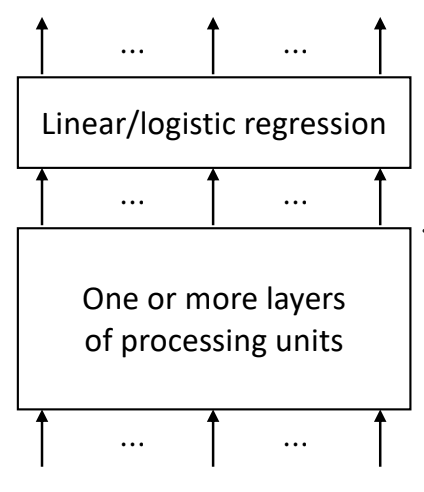
\includegraphics[scale=0.5]{img/FNN1.png}
\end{center}
\end{enumerate}
\subsection{Universal Approximation}
\begin{enumerate}
\item Analogous to \textbf{Turing machine} as a universal mathematical model of computation for today's digital computers, one would also like to know the universal mathematical model for feedforward neural networks.
\item An informal way of stating the universal approximation theorem (proved in the late 1980s) is that, a feedforward neural network with \textbf{sufficiently many sigmoid hidden units in only one layer} can approximate any well-behaved function to arbitrary precision. However, this theorem might have misled people not to put too much effort into exploring deeper neural networks.
\item Nevertheless, using more than one hidden layer may give a network that can approximate the same function using (exponentially) \textbf{fewer parameters} due to the high non-linearly that a deeper network can induce. This higher parameter efficiency also makes deeper networks much \textbf{faster to train}.
\item Deeper networks also mimic better the \textbf{hierarchical organization} of data in many real-world applications.
\end{enumerate}
\subsection{An illustrative example: a 3-layer network}
\begin{enumerate}
\item Each processing unit is shown as a circle. No processing is done in the input layer so no processing units are needed.
\begin{center}
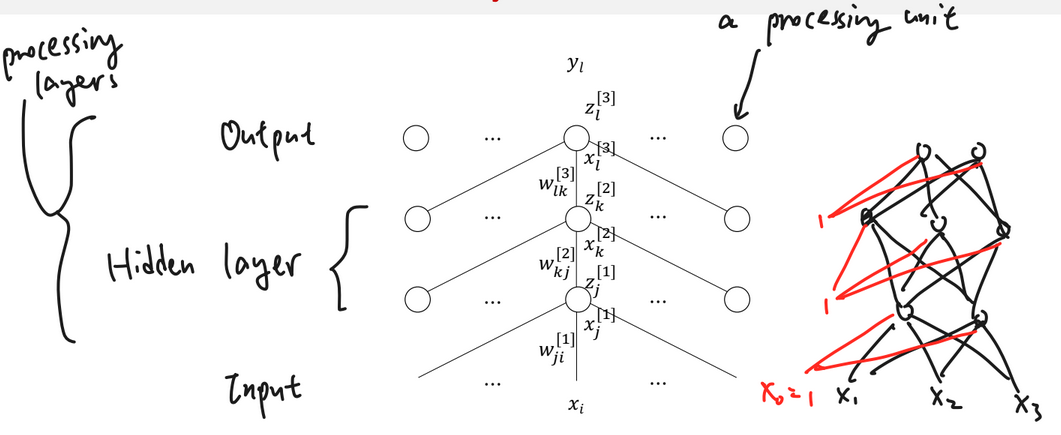
\includegraphics[scale=0.5]{img/FNN2.png}
\end{center}
\item There are \textbf{bias terms} for all the processing layers.
\item We consider here an illustrative example with 2 hidden layers to simply the notation. However, we still call it a 3-layer network as the output layer also count as a layer with processing units.
\item The superscripts, e.g., $[1], [2]$, refer to the corresponding network layers.
\item For each processing unit, 
\begin{enumerate}
\item its (summed) input is denoted by $x^{[*]}$;\\ e.g., $x^{[1]}_{j}$ means the input to $j$-th unit in the first hidden layer.
\item its output is denoted by $z^{[*]}$;\\ e.g., $z^{[1]}_{j}$ means the output from $j$-th unit in the first hidden layer.
\end{enumerate}
\item The input layer may also be denoted using the superscript $[0]$.
\end{enumerate}
\subsection{Activation Functions}
\begin{enumerate}
\item The function relating the input and output of a processing unit is called an activation function of the unit, e.g., $$z_{j}^{[1]} = g_{j}^{[1]}(x^{[1]}_j)$$
\item All the activation functions are \textbf{non-linear}, except for those in the output layer.
\item Note that if the activation functions of the 2 hidden layers are \textbf{linear}, then these 2 layers can be merge into one.
\begin{enumerate}
\item Input layer to first hidden layer: \\Input can be computed by $$x^{[1]}_j = \sum_{i} w^{[1]}_{ji} x_i$$ or in matrix form $$\mathbf{x}^{[1]} = \mathbf{W}^{[1]} \mathbf{x}^{[0]}$$; Output can be computed by $$z_{j}^{[1]} = g^{[1]}_{j} (x^{[1]}_{j})$$ or in matrix form $$\mathbf{z}^{[1]} = g^{[1]}(\mathbf{x}^{[1]})$$
\item First hidden layer to second hidden layer: \\Input can be computed by $$x^{[2]}_j = \sum_{j} w^{[2]}_{kj} z_j$$ or in matrix form $$\mathbf{x}^{[2]} = \mathbf{W}^{[2]} \mathbf{z}^{[1]}$$; Output can be computed by $$z_{k}^{[2]} = g^{[2]}_{k} (x^{[2]}_{k})$$ or in matrix form $$\mathbf{z}^{[2]} = g^{[2]}(\mathbf{x}^{[2]})$$
\item Second hidden layer to output layer: \\Input can be computed by $$x^{[3]}_l = \sum_{k} w^{[3]}_{lk} z_k$$ or in matrix form $$\mathbf{x}^{[3]} = \mathbf{W}^{[3]} \mathbf{z}^{[2]}$$; Output can be computed by $$z_{l}^{[3]} = g^{[3]}_{l} (x^{[3]}_{l})$$ or in matrix form $$\mathbf{z}^{[3]} = g^{[3]}(\mathbf{x}^{[3]})$$
\end{enumerate}
\item[] Sequentially, we can write \begin{align*}
\mathbf{z}^{[3]} &= g^{[3]}(\mathbf{x}^{[3]})\\
&=g^{[3]}(\mathbf{W}^{[3]} \mathbf{z}^{[2]})\\
&= g^{[3]}(\mathbf{W}^{[3]} g^{[2]}(\mathbf{x}^{[2]}))\\
&= g^{[3]}(\mathbf{W}^{[3]} g^{[2]}(\mathbf{W}^{[2]} \mathbf{z}^{[1]}))\\
&= g^{[3]}(\mathbf{W}^{[3]} g^{[2]}(\mathbf{W}^{[2]} g^{[1]}(\mathbf{x}^{[1]})))\\
&= g^{[3]}(\mathbf{W}^{[3]} g^{[2]}(\mathbf{W}^{[2]} g^{[1]}(\mathbf{W}^{[1]} \mathbf{x}^{[0]})))
\end{align*}
If $g^{[1]}$, $g^{[2]}$, and $g^{[3]}$ are linear, we can write $$\mathbf{z}^{[3]} = \mathbf{W}^{[3]}\mathbf{W}^{[2]} \mathbf{W}^{[1]} \mathbf{x}^{[0]} = \mathbf{W'} \mathbf{x}^{[0]}$$, that is, we can merge 3 layers in to one.
\item One exception is in an autoencoder in which a linear function may be used in the hidden units.
\item The logistic function for logistic regression can also seen as an activation function.
\end{enumerate}
\subsection{Loss Functions}
Recall these loss functions:
\begin{enumerate}
\item Squared loss function for regression problems
$$L(\mathbf{W}; \mathcal{S}) = \frac{1}{2} \sum_{q=1}^{N} \sum_{l} (z_{l} ^{[3](q)} - y_{l}^{(q)})^2 = \frac{1}{2} \sum_{q=1}^{N} \sum_{l} (x_{l} ^{[3](q)} - y_{l}^{(q)})^2 $$ The constant $\frac{1}{2}$ is introduced to simplify the subsequent derivation.
\item Cross-entropy loss function for classification problems
$$L(\mathbf{W}; \mathcal{S}) = -\sum_{q=1}^{N} \sum_{l} y^{(q)}_l \log z_{l}^{[3] (q)} = -\sum_{q=1}^{N} \sum_{l} y^{(q)}_l \log \texttt{softmax}(x^{[3] (q)}_l)$$
\end{enumerate}
\subsection{Back-propagation Learning Algorithm}
\begin{enumerate}
\item \textbf{Gradient descent} based on the gradients computed recursively in the backward direction starting from the output layer:
$$\Delta w^{[3]}_{lk} \propto - \pddx{L}{w_{lk}^{[3]}}, \Delta w^{[2]}_{kj} \propto - \pddx{L}{w_{kj}^{[2]}}, \Delta w^{[1]}_{ji} \propto - \pddx{L}{w_{ji}^{[1]}}$$
\item This recursive way of gradient computation for gradient descent is called the back-propagation (BP) learning algorithm.
\item Strictly speaking BP is not a recursive algorithm in the usual programming language sense. They share the same spirit though, e.g., computing $n!$ requires doing something (multiplying by $n$) to the result of $(n-1)!$.
\item More advanced gradient-based learning algorithms may also make use of the gradients computed this way.
\item Algorithm Sketch for (Batch) BP Learning
\begin{algorithm}
    \caption{Batch BP Learning}
    \begin{algorithmic}[1]
        \State Initialize variables
        \Repeat
        	\For {each training example $\mathbf{x}$} 		       		
        		\State predicted-output $\gets$ neural-network-output($\mathbf{x}$) \Comment{Forward propagation}
        		\State actual-output $\gets$ label($\mathbf{x}$)
        		\State Compute error terms at output units by a loss function  
        		\State
        		\State Compute weights changes for last layers of weights ($\Delta w^{[3]}$) \Comment{Backward propagation}
        		\State Compute weights changes for second layers of weights ($\Delta w^{[2]}$)
        		\State Compute weights changes for first layers of weights ($\Delta w^{[1]}$)
        	\EndFor
            \State Update network weights for all layers
        \Until{some stopping criterion is satisfied}
    \end{algorithmic}
\end{algorithm}
\item Gradients computations\\
We first let $$L^{(q)} = \begin{cases} 
\frac{1}{2} \sum_{l} (z_{l}^{[3](q)}-y_{l}^{(q)})^2 \text{ if regression}\\
- \sum_{l} y_{l}^{(q)} \log z_{l}^{[3](q)} \text{ if classification}
\end{cases}$$
\begin{enumerate}
\item Gradients of the last layer of weights $w_{lk}^{[3]}$
\begin{align*}
\pddx{L}{w_{lk}^{[3]}} &= \sum_{q=1}^{N} \pddx{L^{(q)}}{w^{[3]}_{lk}}\\
&= \sum_{q=1}^{N} \pddx{L^{(q)}}{x_{l}^{[3](q)}} \pddx{x^{[3](q)}}{w^{[3]}_{lk}}\\
&= -\sum_{q=1}^{N} \delta^{[3](q)} \pddx{x^{[3](q)}}{w^{[3]}_{lk}}
\end{align*}
So, to compute $\pddx{L}{w_{lk}^{[3]}}$, we need both $\delta^{[3](q)}$ and $\pddx{x^{[3](q)}}{w^{[3]}_{lk}}$
\begin{enumerate}
\item Compute $\delta^{[3](q)}$:
\begin{enumerate}
\item[](for regression)
\begin{align*}
\delta^{[3](q)} &= -\pddx{L^{(q)}}{x_{l}^{[3](q)}}\\
&= -\sum_{m} \pddx{L^{(q)}}{z_{m}^{[3](q)}} \pddx{z_{m}^{[3](q)}}{x_{l}^{[3](q)}}\\
&= - \pddx{L^{(q)}}{z_{l}^{[3](q)}} \pddx{z^{[3](q)}_l}{x^{[3](q)}_{l}}\\
&= y^{(q)}_{l} - z^{[3](q)}_{l}
\end{align*}
\item[] (for classification) 
\begin{align*}
\delta^{[3](q)} &= -\pddx{L^{(q)}}{x_{l}^{[3](q)}} \\
&= -\sum_{m} \pddx{L^{(q)}}{z_{m}^{[3](q)}} \pddx{z_{m}^{[3](q)}}{x_{l}^{[3](q)}}\\
&= \sum_{m} \frac{y_{m}^{(q)}}{z_{m}^{[3](q)}} z^{[3](q)}_{m} (\delta_{ml} - z_{l}^{[3](q)})\\
&= \sum_{m} y_{m}^{(q)} (\delta_{ml} - z_{l}^{[3](q)}) \\
&= y_{l}^{(q)} - z_{l}^{[3](q)}
\end{align*}
\textit{Remarks: the terms $\delta_l ^{[3](q)}$ can be regarded as the error terms computed at the output layer.}
\end{enumerate}
\item Compute $\pddx{x^{[3](q)}}{w^{[3]}_{lk}}$:
$$\pddx{x^{[3](q)}}{w^{[3]}_{lk}} = z_{k}^{[2](q)}$$
\end{enumerate}

\item Gradients of the second layer of weights $w_{kj}^{[2]}$
\begin{align*}
\pddx{L}{w_{kj}^{[2]}} &= \sum_{q=1}^{N} \pddx{L^{(q)}}{w_{kj}^{[2]}}\\
&= \sum_{q=1}^{N} \pddx{L^{(q)}}{x_k ^{[2](q)}}\pddx{x_k ^{[2](q)}}{w_{kj}^{[2]}}\\
&= - \sum_{q=1}^{N} \delta^{[2](q)}_k \pddx{x_k ^{[2](q)}}{w_{kj}^{[2]}}
\end{align*}, where \begin{align*}
\delta^{[2](q)}_k &= - \pddx{L^{(q)}}{x^{[2](q)}_k}\\
&= - \sum_{l} \pddx{L^{(q)}}{x^{[3](q)}_l} \pddx{x^{[3](q)}_l}{z^{[2](q)}_k} \pddx{z^{[2](q)}_k}{x^{[2](q)}_k}\\
&= \sum_{l} \delta^{[3](q)}_l w^{[3]}_{lk} g^{[2]'}_k (x^{[2](q)}_k)
\end{align*}\\ \textit{Remarks: the error terms $\delta_{k}^{[2](q)}$ of the second hidden layer are computed based on $\delta^{[3](q)}_l$}; and $$\pddx{x^{[2](q)}}{w^{[2]}_{kj}} = z_{j}^{[1](q)}$$

\item Gradients of the first layer of weights $w_{ji}^{[1]}$
\begin{align*}
\pddx{L}{w_{ji}^{[1]}} &= \sum_{q=1}^{N} \pddx{L^{(q)}}{w_{ji}^{[1]}}\\
&= \sum_{q=1}^{N} \pddx{L^{(q)}}{x_j ^{[1](q)}}\pddx{x_j ^{[1](q)}}{w_{ji}^{[1]}}\\
&= - \sum_{q=1}^{N} \delta^{[1](q)}_j \pddx{x_j ^{[1](q)}}{w_{ji}^{[1]}}
\end{align*}, where \begin{align*}
\delta^{[1](q)}_k &= - \pddx{L^{(q)}}{x^{[1](q)}_j}\\
&= - \sum_{l} \pddx{L^{(q)}}{x^{[2](q)}_k} \pddx{x^{[2](q)}_k}{z^{[1](q)}_j} \pddx{z^{[1](q)}_j}{x^{[1](q)}_j}\\
&= \sum_{k} \delta^{[2](q)}_k w^{[2]}_{kj} g^{[1]'}_j (x^{[1](q)}_j)
\end{align*}\\ \textit{Remarks: the error terms $\delta_{j}^{[1](q)}$ of the first hidden layer are computed based on $\delta^{[2](q)}_k$}; and $$\pddx{x^{[1](q)}}{w^{[1]}_{ji}} = x^{[1](q)}_i$$
\end{enumerate}
\item Weights Update Rules
\begin{enumerate}
\item Last layer: \begin{align*}
\delta_{l}^{[3](q)} &= y^{(q)}_{l} - z^{[3](q)}_l\\
\Delta w^{[3]}_{lk} &= -\eta \pddx{L}{w^{[3]}_{lk}} = \eta \sum_{q=1}^{N} \delta^{[3](q)}_{l} z^{[2](q)}_k
\end{align*}
\item Second layer: \begin{align*}
\delta_{k}^{[2](q)} &= \sum_{l} \delta^{[3](q)}_l w^{[3]}_{lk} g^{[2]'}_k (x^{[2](q)}_k)\\
\Delta w^{[2]}_{kj} &= -\eta \pddx{L}{w^{[2]}_{kj}} = \eta \sum_{q=1}^{N} \delta^{[2](q)}_k z^{[1](q)}_j
\end{align*}
\item First layer: \begin{align*}
\delta_{j}^{[1](q)} &= \sum_{k} \delta^{[2](q)}_k w^{[2]}_{kj} g^{[1]'}_j (x^{[1](q)}_j)\\
\Delta w^{[1]}_{ji} &= -\eta \pddx{L}{w^{[1]}_{ji}} = \eta \sum_{q=1}^{N} \delta^{[1](q)}_j x^{(q)}_i
\end{align*}
\end{enumerate}
\end{enumerate}
\end{document}